\documentclass[12pt,a4paper]{article}
\usepackage[utf8]{inputenc}
\usepackage[czech]{babel}
\usepackage[T1]{fontenc}
\usepackage{amsmath}
\usepackage{amsfonts}
\usepackage{amssymb}
\usepackage{graphicx}
\usepackage{titlesec}
\usepackage[left=2cm,right=2cm,top=2cm,bottom=2cm]{geometry}
\usepackage{indentfirst}
\usepackage{listings}
\usepackage{color}
\usepackage{array}

%Pravidlo pro řádkování
\renewcommand{\baselinestretch}{1.5}

%Pravidlo pro začínání kapitol na novém řádku
\let\oldsection\section
\renewcommand\section{\clearpage\oldsection}

%Formáty písem pro nadpisy (-změněno na bezpatkové \sffamily z původního \normalfont
\titleformat{\section}
{\sffamily\Large\bfseries}{\thesection}{1em}{}
\titleformat{\subsection}
{\sffamily\large\bfseries}{\thesubsection}{1em}{}
\titleformat{\subsubsection}
{\sffamily\normalsize\bfseries}{\thesubsubsection}{1em}{}

%Nastavení zvýrazňování kódu v \lslisting
\definecolor{mygreen}{rgb}{0,0.6,0}
\definecolor{mygray}{rgb}{0.5,0.5,0.5}
\lstset{commentstyle=\color{mygreen},keywordstyle=\color{blue},numberstyle=\tiny\color{mygray}}

\author{Jan Šmejkal}

\begin{document}

%-------------Úvodni strana---------------
\begin{titlepage}


\includegraphics[width=50mm]{img/FAV.jpg}
\\[160 pt]
\centerline{ \Huge \sc KIV/NET - Programování v prostředí .NET}
\centerline{ \huge \sc Semestrální práce }
\\[12 pt]
{\large \sc
\centerline{Finger Finder - analyzátor otisků prstů}
}


{
\vfill 
\parindent=0cm
\textbf{Jméno:} Štěpán Ševčík\\
\textbf{Osobní číslo:} A13B0443P\\
\textbf{E-mail:} kiwi@students.zcu.cz\\
\textbf{Datum:} {\large \today\par} %datum

}

\end{titlepage}

%------------------------------------------

Souhlasím s vystavením této semestrální práce na stránkách katedry informatiky a výpočetní techniky a jejímu využití pro prezentaci pracoviště.
\begin{flushright}
Štěpán Ševčík
\end{flushright}

%------------------Obsah-------------------
\newpage
\setcounter{page}{2}
\setcounter{tocdepth}{3}
\tableofcontents
%------------------------------------------

%--------------Text dokumentu--------------


\section{Zadání}
Desktopová aplikace v programovacím jazyce C\# umožňující analýzu a klasifikaci otisků prstů

\subsection{Upřesnění požadavků na aplikaci}

\paragraph{Aplikace umožní:}
\begin{itemize}
\item načítání nenormalizovaných snímků otisků prstů z fyzického média.
\item rozpoznání neobvyklých elementů na otisku prstu, takzvaných markantů, a klasifikaci otisku do jedné z možných kategorií \footnote{Samotná analýza a klasifikace je rozsáhlé téma probírané do hloubky v rámci jiného předmětu. Implementace metod v této semestrální práci proto zahrnuje pouze okrajové náhledy do problematiky.}
\item úpravy a doladění detekovaných hodnot
\item ukládání a načítání informací o otisku prstu pro možné porovnávání
\end{itemize}

\section{Analýza zadání}
\subsection{Načítání snímků otisků prstů}
Výběr zdrojového obrázku zajistí hotové nástroje prostředí .NET. Pro zajištění výběru správného typu souboru poslouží poskytnutý filtr, nicméně nelze zajistit že se na vstup dostanou pouze obrázky s otisky prstů. Aplikace bude spoléhat že uživatel vždy vybere pouze obrázek s otiskem prstu a nebude rozlišovat různé stavy.
\subsection{Analýza načteného snímku}
Samotné zkoumání načteného otisku prstu je složitý úkon a je prakticky nemožné analyzovat daný snímek v jeho původní podobě protože se často stane, že snímek není zachycen v ideálních podmínkách. Z toho důvodů se nejdříve snímek podrobí procesu předzpracování a analýza se provádí až nad upraveným snímkem.
\par
Otisku prstu také může být zachycen různými způsoby a různé snímky nemusí být zpracovatelné stejným postupem a proto je potřeba postup předzpracování implementovat obecně.
\subsection{Úpravy a doladění detekovaných hodnot}
Prostřednictvím komponent prostředí Windows Presentation Foundation bude uživateli umožněna kontrola detekovaných údajů a jejich případná úprava přímo v rámci stejného pohledu.
\subsection{Ukládání a načítání údajů o otisku prstu}
Nezbytné údaje, které je nutné udržovat, jsou informace o jednotlivých nalezených markantech, detekovaná kategorie otisku prstu a popisek pro identifikaci.

Pro vizuální kontrolu se také uchovávají předzpracované snímky a pro případnou možnost řazení se uchovává datum sejmutí otisku.

\section{Implementace}
\subsection{Předzpracování}
Předzpracování načteného snímku otisku prstu nelze definovat jednotně z důvodu různorodosti metod zachycení snímku otisku prstu. Všeobecný postup předzpracování se dá přirovnat ke stavovému automatu: předzpracování se vždy nachází v určitém stavu (v našem případě v určité fázi) a mezi fázemi se pohybuje po hranách použitím vstupů(zde použitím transformací obrázku). Obecný postup tedy vypadá následovně:
\begin{enumerate}
\item[1] Načti obrázek a nastav fázi na k = 1
\item[2] Aplikuj k. transformaci a nastav fázi na k = k + 1
\item[3] Pokud fáze k neodpovídá finální fázi N, opakuj krok 2
\item[4] Dokonči předzpracování a přejdi na analýzu
\end{enumerate}
V této semestrální práci je předdefinován pouze jeden postup předzpracování metodou skeletizace ale v rámci obecného řešení je aplikace připravená na další metody předzpracování, což zahrnuje možnost výběru metody po načtení obrázku a obecný průchod postupem předzpracování.

\subsubsection{Skeletizace}
Metoda skeletizace je založená na rozlišení rozdílů v obrazové matice po základních směrech.
\paragraph{Ekvalizace histogramu}
Prvním krokem předzpracování je ekvalizace, což znamená zjištění jasového spektra, které nemusí být v základu rozložené po celém použitelném intervalu jasového spektra, a jeho roztažení. Tento krok usnadňuje následující krok, prahování.
\paragraph{Prahování}
Tato transformace vyžaduje určení hrany v jasovém spektru, neboli prahu, podle které se každá jasová úroveň změní buď na bílou nebo na černou. Tento krok umožňuje rozpoznávání tvarů.
\paragraph{Skeletizace}
V tomto kroku se pomocí sofistikovaného algoritmu z ekvalizovaného snímku vytvoří kostra reprezentující jednotlivé papylární linie.

\subsection{Datový model}
\subsubsection{Otisk prstu}
Každý záznam otisku prstu je sám o sobě plnohodnotný a není potřeba k němu vést doplňující záznamy. Záznamy otisku prstu schraňují tyto informace:
\begin{itemize}
\setlength\itemsep{-0.3cm}
\item Textový popis
\item Datum sejmutí otisku
\item Kategorie otisku prstu
\item Seznam nalezených markantů
\end{itemize}
V rámci serializace se struktura otisku prstu obaluje do nosiče, ve kterém se dále schraňují tyto informace:
\begin{itemize}
\setlength\itemsep{-0.3cm}
\item Verze aplikace při uložení
\item Cesta k obrázku
\end{itemize}
\subsubsection{Markant}
Informace o markantu se skládají z následujících položek:
\begin{itemize}
\setlength\itemsep{-0.3cm}
\item Pozice
\item Typ markantu
\end{itemize}
\paragraph{Typ markantu} je výčet typů markantů a slouží k definování kategorií do kterých může markant spadat.
\subsubsection{Kategorie otisku prstu}

Otisk prstu lze klasifikovat do jedné z kategorií definovaných tímto výčtem.


\section{Struktura aplikace}
Výkonná část programu je oddělená v samostatné knihovně tříd, což umožňuje znovupoužitelnost a relativně jednoduché obměňování uživatelského rozhraní.

\subsection{Výkonná část}
\subsubsection{Před-zpracovatel}
Logický celek obstarávající sekvenční zpracování obrázku. Poskytuje rozhraní pro krokování mezi fázemi a uchovává průběžné mezivýsledky jednotlivých kroků před-zpracování.

Jednotlivé transformace jsou zpracovávány specifickými manipulátory.
\subsubsection{Analyzátor}
V této třídě se uchovává obrázek otisku prstu v jeho finální podobě. Nad tímto snímkem se touto třídou vyvolávají analyzující procesy. Dále tato třída zprostředkovává načítání a ukládání záznamů o otiscích prstů.

\subsubsection{XML exportér / importér záznamu o otisku}
Tato třída se stará o serializaci respektive de-serializaci záznamu o otisku prstu. Laicky řečeno ukládá informace o otisku prstu do souboru nebo je naopak ze souboru načítá. \par

K ukládání informace o verzi programu využívá obalující třídu neboť standardní verze ukládání serializací nepodporuje.

\subsubsection{Manipulátory obrázku}
Manipulátory jsou třídy dedikované určité transformaci neboli přeměně, například ekvalizaci histogramu. Neboť všechny manipulátory fungují typově stejně, tedy převádí obrázek na upravený obrázek, jsou sloučeny pod společnou abstraktní třídu, která zvyšuje znovupoužitelnost. Tato abstraktní třída také zajišťuje jednotné deklarace všeobecných konstant a sjednocení stejných transformací, například tříprvkové barvy na jednoprvkovou 'světlost'.

Pro možnost konfigurace transformace lze argumentem předat i dynamickou instanci obsahující parametry specifické pro jednotlivé transformace.

\subsection{Uživatelské rozhraní}
Jakožto uživatelské rozhraní bylo zvoleno prostředí WPF (Windows Presentation Foundation) pomocí kterého lze jednoduše deklarovat ovládací prvky.

Rozhraní je definované v jednom souboru a obsahuje jediný datový kontext. V tomto kontextu jsou deklarovány potřebné instance pro předzpracování a analýzu. Data jsou do tohoto rozhraní provázána přímo nebo jsou transformována převodníky.

\section{Uživatelská příručka}
Uživatelské prostředí umožňuje vytváření nových údajů importováním z obrázku anebo načítání již existujících záznamů.
Tyto záznamy lze v rámci prostředí modifikovat a také je lze ukládat na požadované místo v rámci souborového systému.
\subsection{Základní pohled}
Po spuštění se program nachází v úvodním pohledu, kde informuje uživatele o možnostech.
\begin{figure}[h]
  \centering
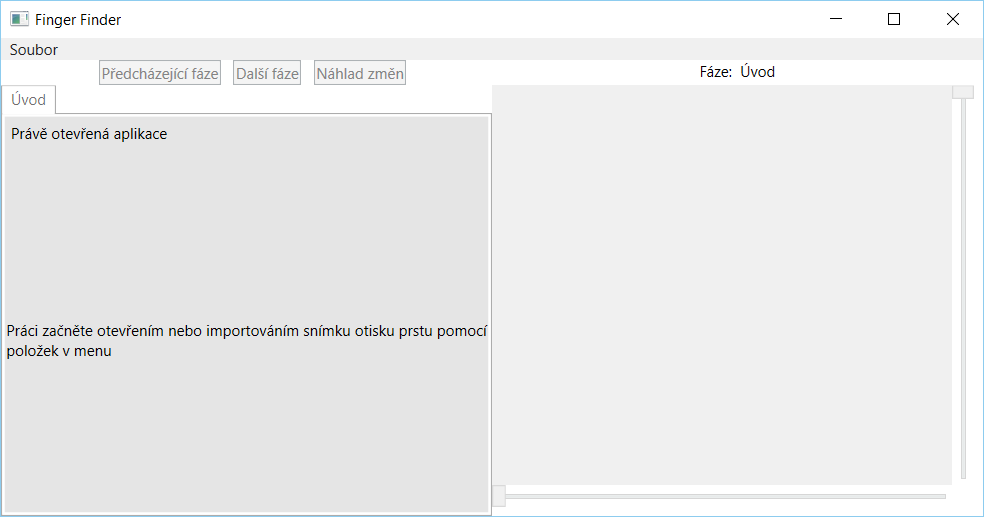
\includegraphics[width=120mm]{img/um_01_intro.png}
  \caption{Úvodní pohled}
\end{figure}
Zde může uživatel pomocí menu importovat obrázek a přejít do režimu předzpracování anebo načíst údaje otisku prstu a přejít přímo do režimu analýzy.

\newpage
\subsection{Pohled před-zpracování}
V režimu předzpracování má uživatel na výběr z dostupných způsobů předzpracování, v této verzi je dostupné pouze předzpracování metodou skeletizace.


\begin{figure}[h]
  \centering
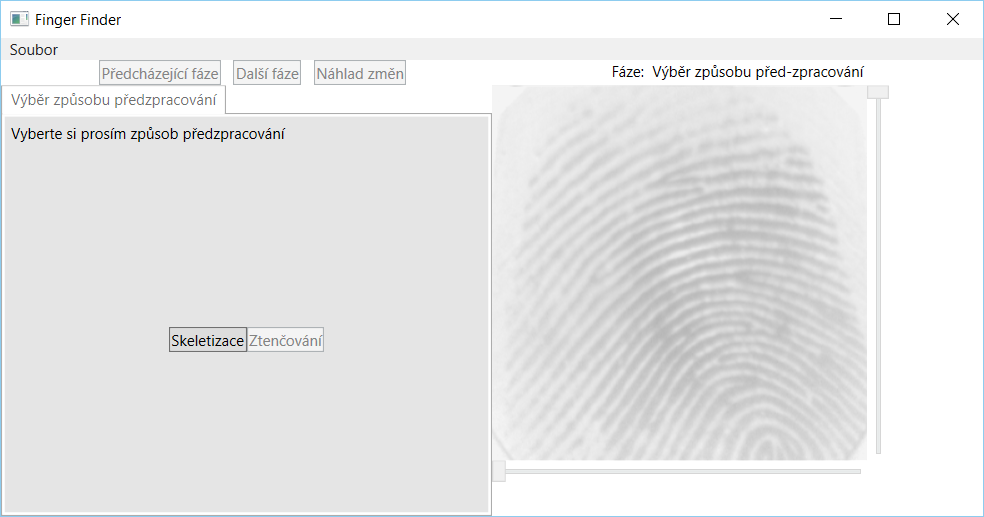
\includegraphics[width=120mm]{img/um_02_preprocess.png}
  \caption{Výběr metody předzpracování}
\end{figure}
Navigace mezi kroky je umožněna odpovídajícími tlačítky, které se aktivují podle validity jejich významu, tedy například pokud je uživatel na začátku předzpracování, nemůže vykonat krok zpět.
\begin{figure}[h]
  \centering
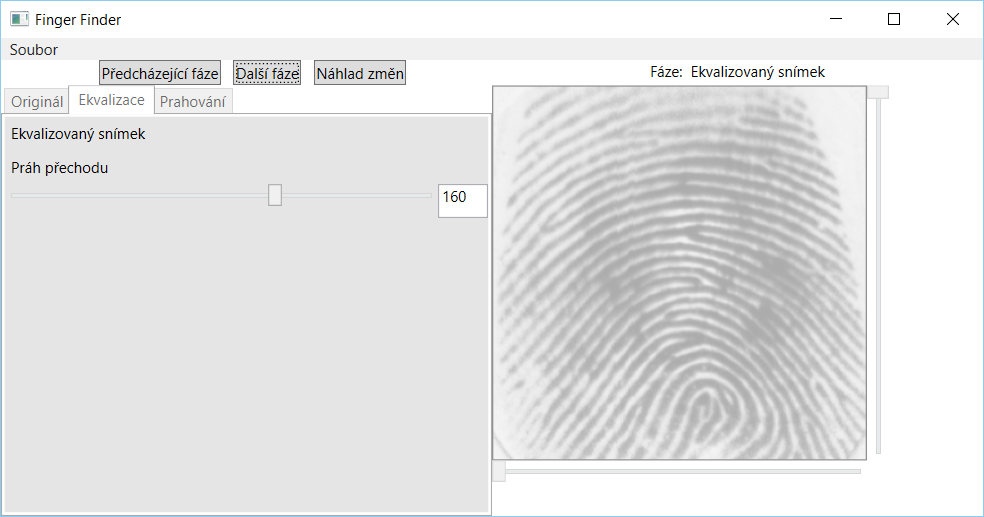
\includegraphics[width=120mm]{img/um_03_steps.png}
  \caption{Příklad kroku předzpracování s parametrem}
\end{figure}
V některých krocích je možné určovat parametry transformace pomocí kontrolek, jako například v kroku prahování posuvníkem. Uživatel si před krokem na další fázi v takovémto případě může ověřit správnost konfigurace transformace zobrazením náhledu.

\subsection{Pohled analýza}
Finálním krokem aplikace je pohled analýza, kde může uživatel spouštět proces hledání markantů a klasifikaci otisku. Detekované hodnoty také může následně doladit pomocí poskytnutých kontrolek.

\begin{figure}[h]
  \centering
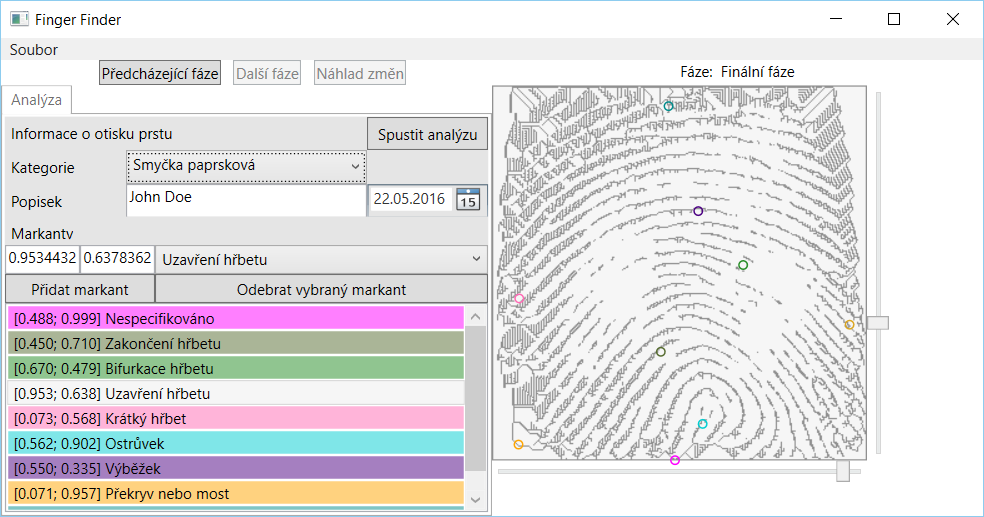
\includegraphics[width=120mm]{img/um_04_analyse.png}
  \caption{Příklad kroku předzpracování s parametrem}
\end{figure}
\section{Závěr}
Při vytváření aplikace jsem se snažil dbát na obecnost řešení ve většině oblastí ale s kolegou jsme se ve fázi analýzy zadáni neponořili dostatečně hluboko do problematiky. Toto vedlo k neohrabanému řešení fáze předzpracování, které bylo potřeba refaktorovat za účelem oddělení logiky a možnosti obměňování postupů předzpracování.
Další z problémů, na které jsem při vytváření narazil byla vizualizace informací, se kterými program manipuluje, v rámci prostředí Windows Presentation Foundation. V určité fázi vývoje jsem se potýkal s nepředvídatelným chováním vykreslování pozadí plátna, na které se vykreslují kružnice reprezentující markanty. Tuto skulinu jsem byl nucen obejít implicitním roztahováním pozadí a proměnlivou velikostí plátna.

Tento program se odchýlil od původního zadání, vytvoření programu, který analyzuje obrázek, a výsledný produkt je prostředí umožňující a značně usnadňující tyto manipulace. Důvodem pro toto odchýlení bylo omezení spolupráce, přičemž řešení této problematiky je škálováno pro alespoň dva vývojáře.

\section*{Programátorský deník}
Tato sekce nezahrnuje všechna sezení nad touto prací neboť jsem si vždy nevzpomněl spustit časovač a také protože na některých částech pracoval spolu-autor.
\begin{table}[h!]
\centering
\begin{tabular}
{| c | >{\centering}m{12cm} | c |} \hline
Datum & Aktivita & Délka \\ \hline

03.04. & Návrh WinForms vzhledu UI & 1:20 \\ \hline
03.04. & Načítání a vykreslování obrázků & 0:40 \\ \hline
17.04. & Export / import & 1:30 \\ \hline
17.04. & Úprava WPF - nástrojová struktura & 1:20 \\ \hline
18.04. & Refaktorizace struktury - postupné zpracování & 2:00 \\ \hline
23.04. & Dokumentace & 4:00 \\ \hline
02.05. & Refaktorizace modelu & 3:30 \\ \hline
03.05. & Parametrizace transformací & 0:40 \\ \hline
04.05. & Editace a zobrazování markantů & 2:10 \\ \hline
12.05. - 14.05. & Zobecnění postupu předzpracování & 10:30 \\ \hline
14.05. & Refaktorizace manipulátorů & 2:40 \\ \hline
15.05. & Vykreslování markantů & 1:30 \\ \hline
15.05. & Export-Import a čištění kódu & 4:40 \\ \hline
16.05. & Vykreslování markantů & 6:50 \\ \hline
18.05. & Vykreslování markantů a čištění kódu & 1:20 \\ \hline
20.05. & Implementace verze do XML souboru & 0:30 \\ \hline
21.05. & Refaktorizace výčtů umožňující překlad & 1:00 \\ \hline
22.05. & Dokumentace & 3:20 \\ \hline


\hline
 & \textbf{Celkem} & \textbf{49:30} \\ \hline

\end{tabular}
\end{table}

%------------------------------------------

\end{document}
